\documentclass[nooutcomes,handout]{ximera}
\usepackage{fullpage}
%% handout
%% space
%% newpage
%% numbers
%% nooutcomes

\newcommand{\RR}{\mathbb R}
\renewcommand{\d}{\,d}
\newcommand{\dd}[2][]{\frac{d #1}{d #2}}
\renewcommand{\l}{\ell}
\newcommand{\ddx}{\frac{d}{dx}}
\newcommand{\dfn}{\textbf}
\newcommand{\eval}[1]{\bigg[ #1 \bigg]}

\usepackage{multicol}

\renewenvironment{freeResponse}{
\ifhandout\setbox0\vbox\bgroup\else
\begin{trivlist}\item[\hskip \labelsep\bfseries Solution:\hspace{2ex}]
\fi}
{\ifhandout\egroup\else
\end{trivlist}
\fi} 

\title{4.5: Linear Approximation and Differentials}

\begin{document}
\begin{abstract}
\end{abstract}
\maketitle

%problem1
\begin{problem}


  \begin{enumerate}
    \item
      Find the linearization, $L(x)$, of the function $f(x) = e^{2x}$ at $a = 0$.
      \begin{freeResponse}
        Recall that $L(x) = f(a) + f'(a)(x - a)$.\\
        Hence  $f'(x) = 2e^{2x} \implies f'(0) = 2e^{0} = 2$  and $ f(0) = e^{0} = 1$.\\
        Therefore $L(x) = 1 + 2\cdot x$
      \end{freeResponse}

    \item
    Using the linearization, $L(x)$, from the part (a), approximate $e$.
      \begin{freeResponse}
        \begin{align*}
          e &= e^{2\cdot(1/2)}\\
          &= f(1/2) \approx L(1/2)\\
          &\approx 1 + 2\cdot(1/2)\\
          &\approx 2
        \end{align*}
      \end{freeResponse}

  \end{enumerate}
\end{problem}

%problem 2
\begin{problem}

Complete steps (i)-(vii) below in order to estimate the following values using linear approximation:
\begin{enumerate}
	\item $\cos \left( \frac{31 \pi}{180} \right)$	
	\item $\sqrt[3]{8.13} $
\begin{enumerate}
\item Identify the function, $f(x)$.
\item  Find the nearby value where the function can be easily calculated, $x=a$.
\item Find $\Delta x=dx$.
\item  Find the linear approximation, $L(x)$.  
\item  Compute the approximate value of the expression using the linear approximation.
\item  Compare the approximated value to the value given by your calculator.
\item  Compare $dy$ and $\Delta y$ using the value given by your calculator.
\end{enumerate}
\end{enumerate}

\begin{freeResponse}
\begin{enumerate}
	\item $ \cos \left( \frac{31 \pi}{180} \right)$
  \begin{enumerate}
    \item  $f(x) = \cos x$
    \item $a = \frac{30 \pi}{180} = \frac{\pi}{6}$
    \item  $\Delta x = \frac{31 \pi}{180} - \frac{\pi}{6} = \frac{\pi}{180}$
    \item
    \begin{align*}
      L(x) &= f\left( \frac{\pi}{6} \right) + f^\prime \left(\frac{\pi}{6} \right) \left( x - \frac{\pi}{6} \right) \\
           &= \cos \left( \frac{\pi}{6} \right) - \sin \left(\frac{\pi}{6} \right) \left( x - \frac{\pi}{6} \right) \\
           &= \frac{\sqrt{3}}{2} - \frac{1}{2} \left( x - \frac{\pi}{6} \right) 
    \end{align*}
    \item 
    \begin{align*}
      L \left( \frac{31 \pi}{180} \right) &= \frac{\sqrt{3}}{2} - \frac{1}{2} \left( \frac{31 \pi}{180} - \frac{\pi}{6} \right) \\
                                          &=  \frac{\sqrt{3}}{2} - \frac{1}{2} \left( \frac{\pi}{180} \right) \\
                                          &= \frac{1}{2} \left( \sqrt{3} - \frac{\pi}{180} \right) \\
                                          &\approx 0.857299
    \end{align*}
    \item  $\cos \left( \frac{31 \pi}{180} \right) \approx 0.857167$
    \item
      $$ dy = L\left( \frac{31\pi}{180} \right) - L \left( \frac{\pi}{6} \right) \approx -0.008727 $$
      $$ \Delta y = \cos \left( \frac{31 \pi}{180} \right) - \cos \left( \frac{\pi}{6} \right) \approx -0.008858 $$
  \end{enumerate}
  
  \item $ \sqrt[3]{8.13}$
  \begin{enumerate}
    \item  $f(x) = \sqrt[3]{x}$.
    \item  $a=8$.
    \item  $\Delta x = 8.13 - 8 = 0.13$.
    \item 
      \begin{align*}
        L(x) &= f(8) + f^\prime (8) (x-8) \\
             &= \sqrt[3]{8} + \frac{1}{3 (\sqrt[3]{8})^2} \left( x - 8 \right) \\
            &= 2 + \frac{1}{12} (x-8) 
      \end{align*}
    \item  
      \begin{align*}
        L(8.13) &= 2 + \frac{1}{12} (8.13 - 8) \\
                &= 2 + \left( \frac{1}{12} \right) \left( \frac{13}{100} \right) \\
                &= 2 + \frac{13}{1200} = \frac{2413}{1200} \\
                &\approx 2.010833
      \end{align*}
    \item  $\sqrt[3]{8.13} \approx 2.010775$.
    \item  
      $$ dy = L(8.13) - L(8) \approx 0.010833 $$
      $$ \Delta y = \sqrt[3]{8.13} - \sqrt[3]{8} \approx 0.010775 $$
    \end{enumerate}
    \end{enumerate}
\end{freeResponse}
\end{problem}

%problem 3
\begin{problem}

  Consider the graph of $f^\prime (x)$ given below.
  Suppose that $f(2) = 4$.
  Approximate $f(1.98)$ and $f(2.02)$ as best as you can.
  Determine whether your approximations are over or under estimates.
  Suppose you also know $f(3) = 7$.
  Can you approximate $f(2.98)$ and $f(3.02)$?
  Explain your answer.
  \begin{center}
    \begin{image}
      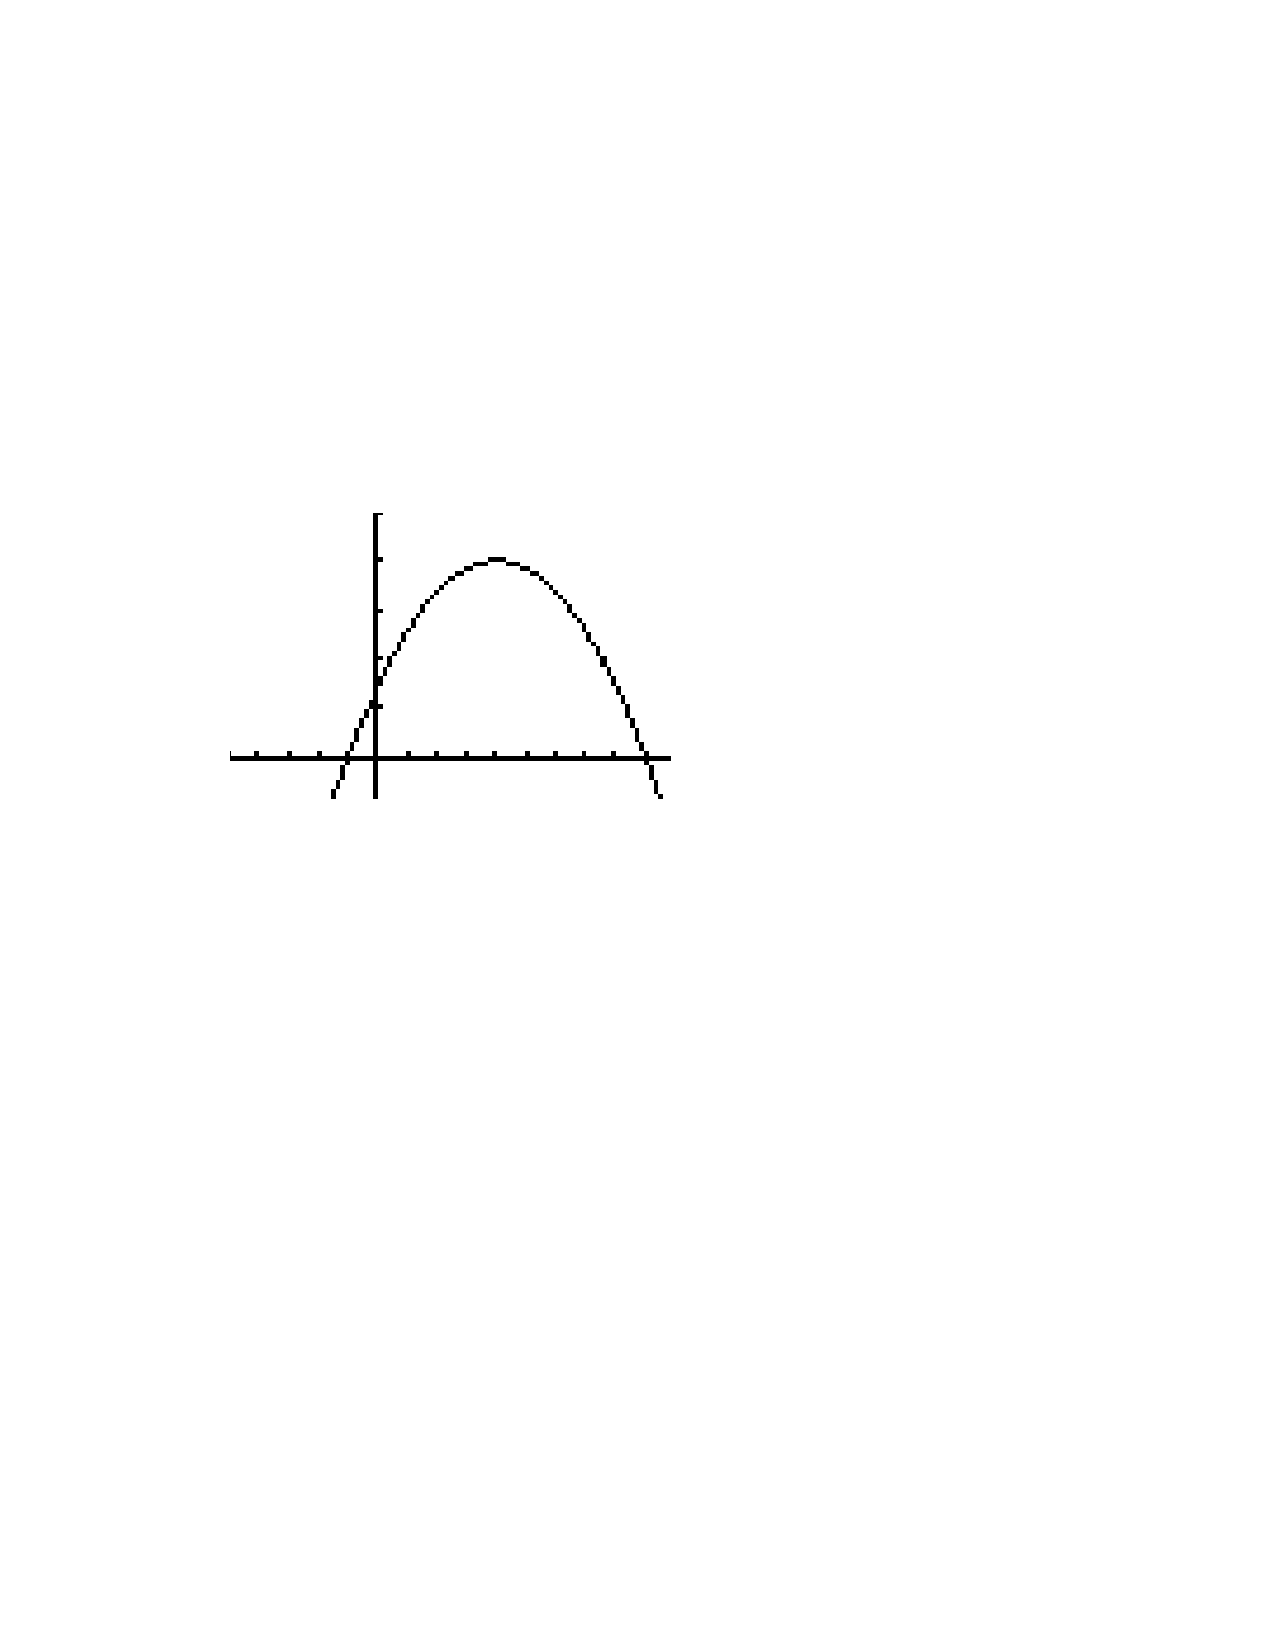
\includegraphics{Figure1.png}
    \end{image}
  \end{center}
  \begin{freeResponse}
    $f(2) = 4$ and $f^\prime (2)$ looks to be about $1.75 = \frac{7}{4}$.
    So $L(x) = 4 + \frac{7}{4} (x-2)$.
    Therefore
    \begin{align*}
      L(1.98) &= 4 + \frac{7}{4} (1.98-2) = 4 + \frac{7}{4} (-0.02) = 4-0.035 = 3.965 \\
      L(2.02) &= 4 + \frac{7}{4} (2.02-2) = 4 + \frac{7}{4} (0.02) = 4+0.035 = 4.035
    \end{align*}
    So $f(1.98)\approx 3.965$ and $f(2.02)\approx 4.035$ 
    Since $f^\prime$ is decreasing, the graph of $f$ is concave down.
    Therefore the graph of $L(x)$ lies above the graph of $f$ near $x=2$.
    This means that these are overestimates.

    $f(3)=7$ and $f^\prime (3)=0$ 
    $$ L(x) =7+0(x-3) = 7$$
    This is a constant function, and so our approximations are $f(2.98)\approx 7$ and $f(3.02)\approx 7$.
    These are overestimates for the same reason as before.
  \end{freeResponse}
\end{problem}

%problem 4
\begin{problem}

  Estimate the amount of paint needed to apply a coat of paint $.05$ cm thick to a hemispherical dome with diameter $50$m.
 
  \begin{freeResponse}
    The radius of the dome is $\frac{50}{2}m=25m$.
    The paint increases this by 0.0005m (0.05cm to meters).
    The volume of a ``hemispherical dome'' (or half of a sphere) is $V = \frac{1}{2} \left(\frac{4}{3} \pi r^3 \right) = \frac{2}{3} \pi r^3$.
    Then
    $$ \d V = 2 \pi r^2 \d r  $$
    The amount of paint needed is approximately the change in volume ($\d V$).
    We also have that $r=25m$ and $\d r = (5 \times 10^{-4}) m$.
    Thus, the amount of paint needed to paint the dome is approximately
    $$ \eval{\d V}_{r=25,\d r = 0.0005} = 2 \pi (25)^2 (5 \times 10^{-4}) = 5 \pi (0.125) = 0.625 \pi \approx 1.9635 m^3$$
    
 
  \end{freeResponse}
\end{problem}





%problem 5
\begin{problem}
The graph of a function $f$ is given below.
    \begin{image}
      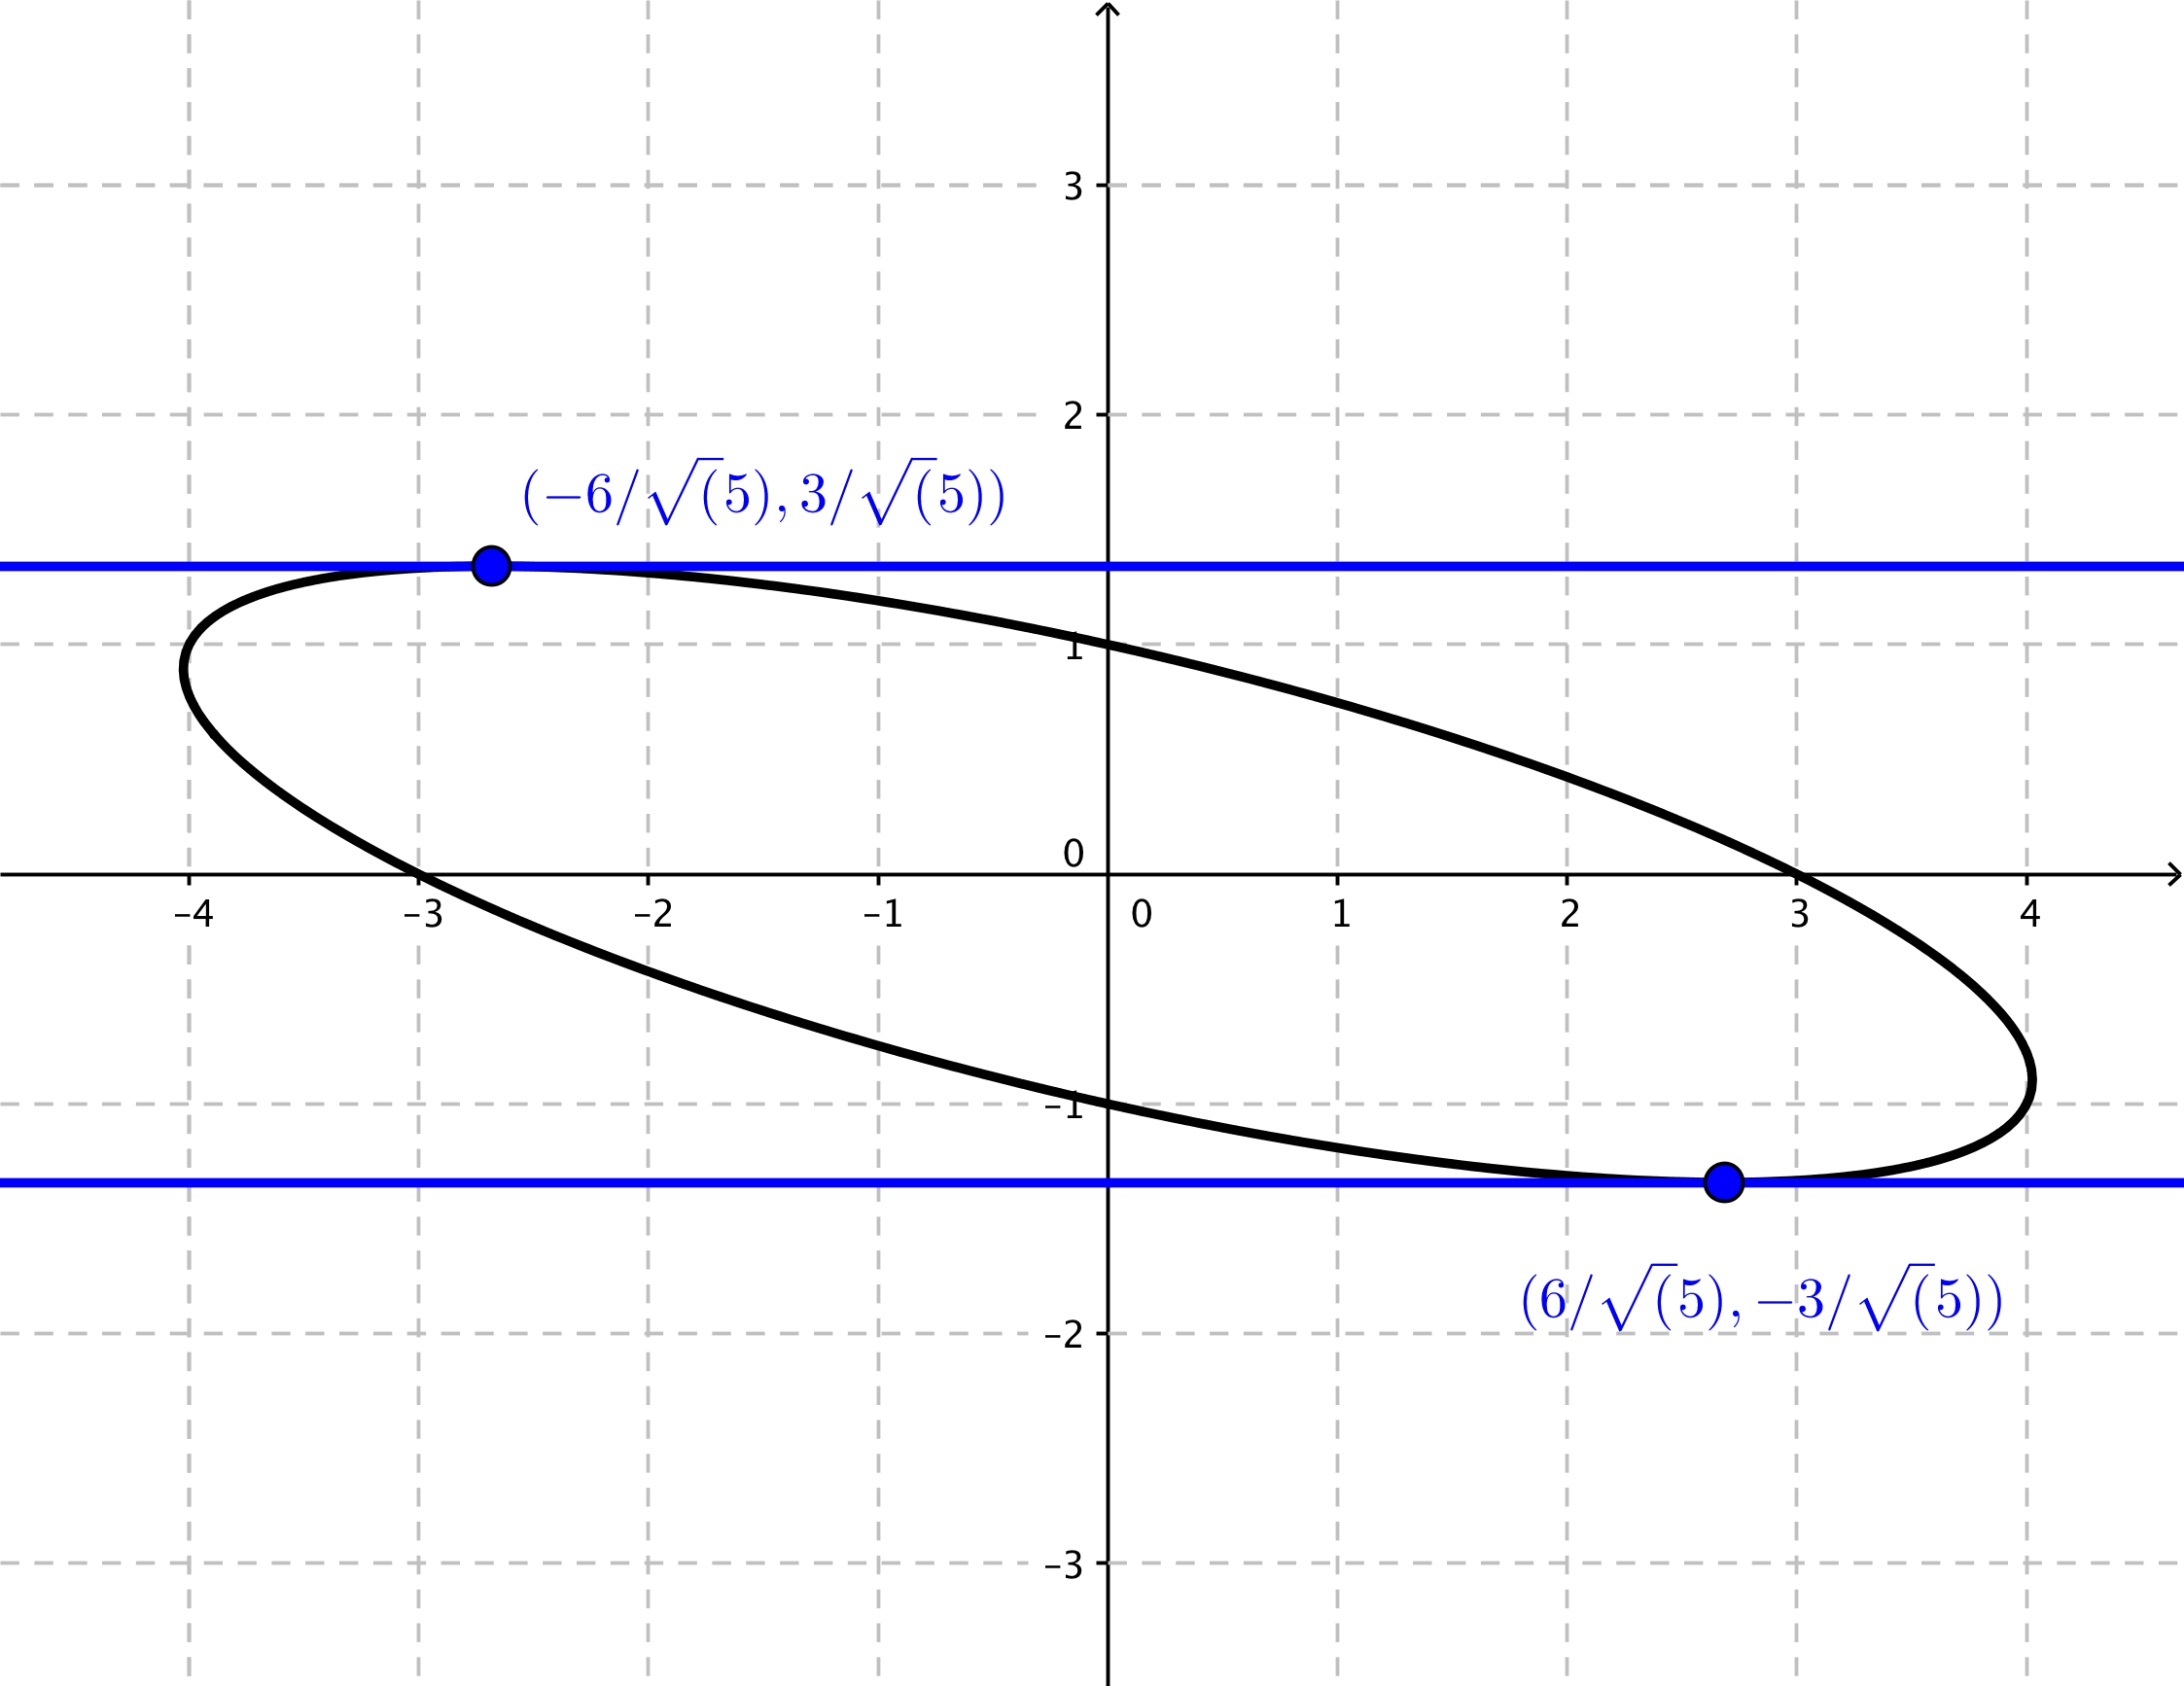
\includegraphics[scale = .7]{figure3.png}
    \end{image}
\begin{enumerate}

%part a
\item Given that $f'(2)=1$, find the linear approximation $L$ to the function $f$ at $a=2$.

\begin{freeResponse}
$L(x)=f(2)+f'(1)(x-2)=2+(x-2)=x$
\end{freeResponse}

%part b
\item Sketch the graph of $L$ in the figure above.
\begin{freeResponse}
    \begin{image}
      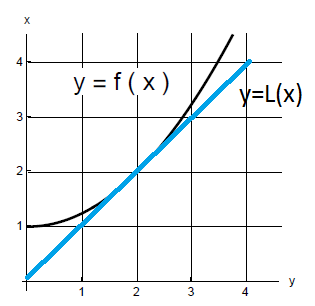
\includegraphics[scale = .7]{figure4.png}
    \end{image}
\end{freeResponse}

%part c
\item Use the linear approximation $L$ to estimate the value of $f(3)$.  Is this an underestimate or overestimate?  Explain.
\begin{freeResponse}
$f(3)\approx L(3)=3$.  It is an underestimate because $L(x)<f(x)$ since $f$ is concave up.
\end{freeResponse}

%part d
\item When $x$ changes from $a=2$ to $a+\Delta x=3$, the change in the {\bf function} $y=f(x)$, $\Delta y$, is given by $\Delta y=f(a+ \Delta x)-f(a)$.  Draw and label $\Delta y$ and $\Delta x$ in the figure above.

\begin{freeResponse}
   \begin{image}
      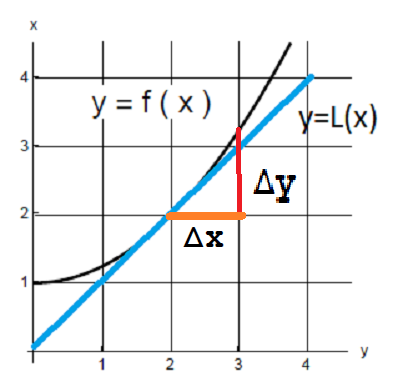
\includegraphics[scale = .6]{figure5.png}
    \end{image}
\end{freeResponse}

%part e
\item When $x$ changes from $a=2$ to $a+ \Delta x=3$, the change in the {\bf linear approximaton}, $dy$, is given by $dy=L(a+\Delta x)-L(a)=f'(a)\Delta x$.  Draw and label $L(x)$, $dx$ and $dy$ (differential) in the figure above.
   \begin{image}
      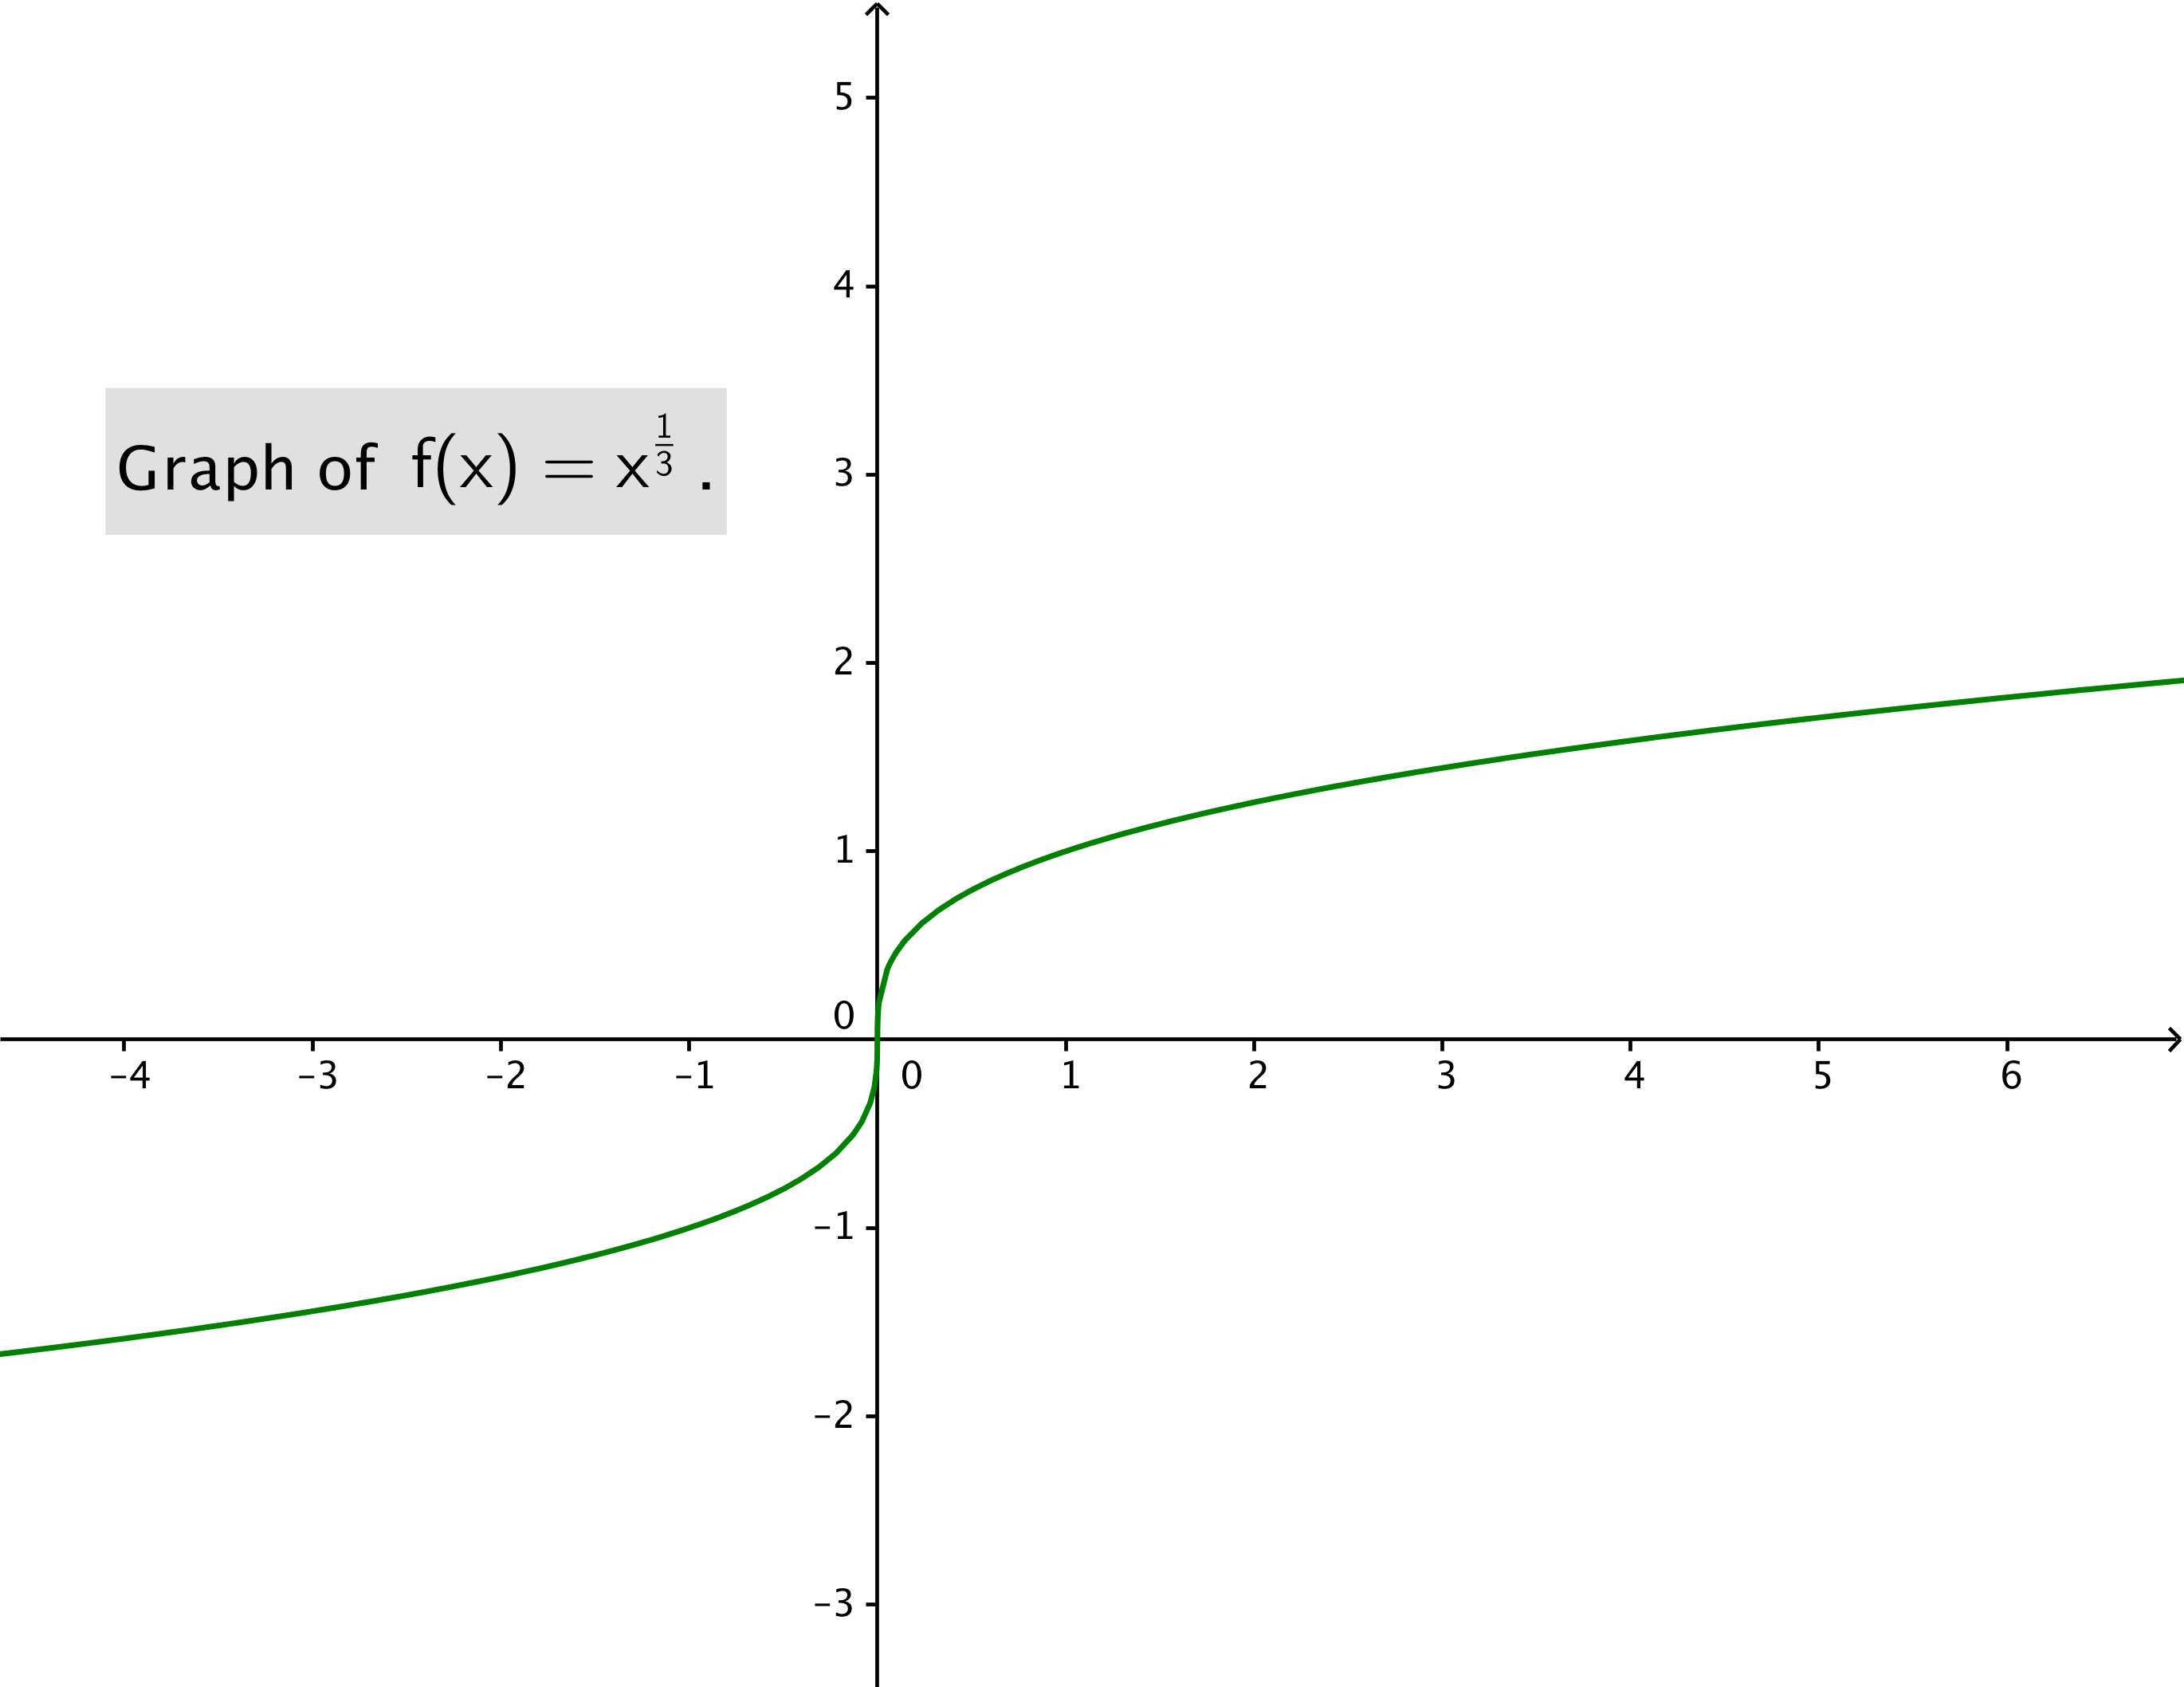
\includegraphics[scale = .7]{figure6.png}
    \end{image}
\begin{freeResponse}
   \begin{image}
      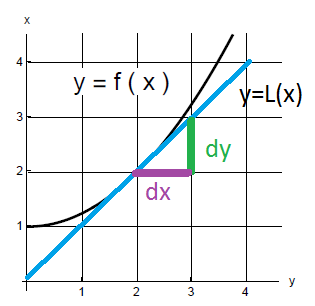
\includegraphics[scale = .7]{figure7.png}
    \end{image}
\end{freeResponse}

\end{enumerate}
\end{problem}

%problem 6
\begin{problem}

  The figure shows the graph of a function $f$.
  Let $L_a(x)$ be the linear approximation of $f$ at $a$.
  \begin{image}
    \includegraphics[scale = 1]{"Linear approximation graph".png}
  \end{image}
  Circle ALL the correct statements below.
  \begin{enumerate}
    \item
      $L_a(b) < f(b)$
    \item
      $L_a(b) > f(b)$
    \item
      $L_a(a) < f(a)$
    \item
      $L_a(a) > f(a)$
    \item
      No statement (a)~--~(d) is correct.
  \end{enumerate}
  \begin{freeResponse}
    From the graph of $f$ and the the graph of $L_a(x)$ we see that the correct statement is (a):
    \begin{image}
      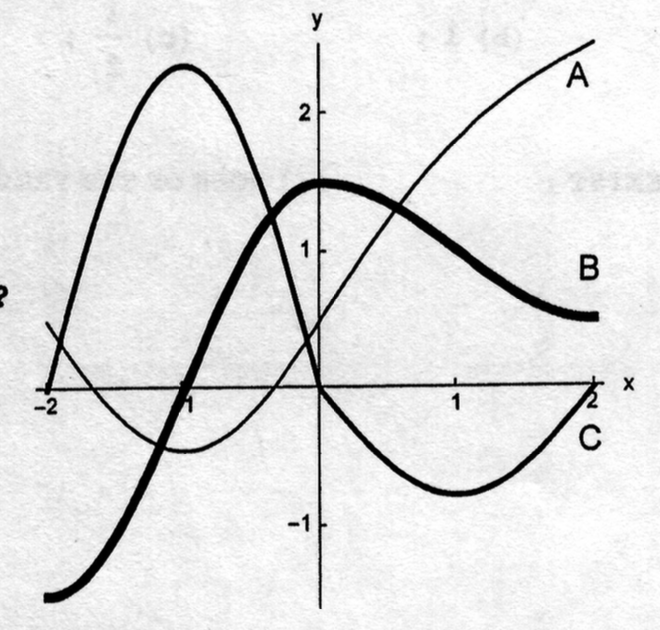
\includegraphics[scale = .5]{figure2.png}
    \end{image}
  \end{freeResponse}
\end{problem}

%problem 7
\begin{problem}

  By using linear approximation, determine which of the following is the best estimate of $e^{0.002}$.
  \begin{enumerate}
    \item1.00100050016679834166
    \item 1.00200200133400026675
    \item 1.00300450450337702601
    \item 1.02020134002675581016
  \end{enumerate}
  \begin{freeResponse}
    Let $f(x) = e^x$ and $a=0$.  Then since $f'(x) = e^x$, we have that
    \begin{align*}
      L(x) &= f(a) + f'(a)(x-a) \\
           &=  f(0) + f'(0)(x-0) \\
           &= e^0 + e^0x \\
           &= 1 + x
    \end{align*}
    Then since $L(0.002) = 1 + 0.002 = 1.002$, the answer is (b).
  \end{freeResponse}	
\end{problem}

\end{document} 
